% !TeX spellcheck = en_US

%TODO Sibel

\begin{comment}
	- second conceptual neighborhood model
	- smooth transition: definition
	- occurrence of smooth transition -> conceptual neighborhood
	\end{comment}

	\begin{frame}{Smooth-Transition Model}
		\begin{block}{Example}
			A pair of line-region relations that are conceptual neighbors (one can be obtained from the other via a ''smooth transition'')
		\end{block}
		
		\begin{block}{Counterexample}
			A pair of line-region relations that \textbf{not} are conceptual neighbors
		\end{block}
	\end{frame}
	
	\begin{frame}{Formalization}
		\begin{block}{Possible Changes} A smooth transition can occur by:
			\begin{itemize}
				\item Moving around a line's boundary nodes
				\begin{itemize}
					\item[Rule 1] Line's two boundary nodes intersect with same region part
					\item[Rule 2] Line's two boundary nodes intersect with different region part
				\end{itemize}
				\item Moving around a line's interior
				\begin{enumerate}
					\item[Rule 3] Extend line's interior-intersection partially
					\item[Rule 4] Reduce line's interior-intersection partially
				\end{enumerate}
			\end{itemize}
		\end{block}
		
%		In terms of 9-Intersection, a smooth transition means that an intersection or its adjacent intersection gets changed from empty to non-empty, or reverse.
	\end{frame}
	
	\begin{frame}{Extent of a Line Part}
		Extent of a part $i$: Denoted by $ \#M[i, \_]$; number of non-empty intersections between $i$ and th three parts of the second object.
		Define extent of a part i Draw 9-intersection model on the board for reference
		
		\begin{itemize}
			\item (Explain on the board) The extent of a line's interior with respect to a region is in the interval of 1 to 3, the extent of the lines boundary is either 1 (if both nodes are located in the same region part) or 2 (if the nodes are located in different parts of the region), and the extent of a line's interior is always 3.
		\end{itemize}
	\end{frame}
	
%	\begin{frame}{First Rule}
%		If the line's two boundaries intersect with the same region part, then extend the intersection to either of the adjacent region parts.
%		\begin{block}{Formalization}
%			\centering $ \#M[\delta, \_] = 1 \Rightarrow
%			\forall i (M[\delta, i] = \NotEmpty):
%			M_{N}[\delta, \text{adjacent}(i)] := \NotEmpty $
%		\end{block}
%		
%		\begin{block}{Example}
%			%Moving one boundary of a line into an adjacent part of the region.
%			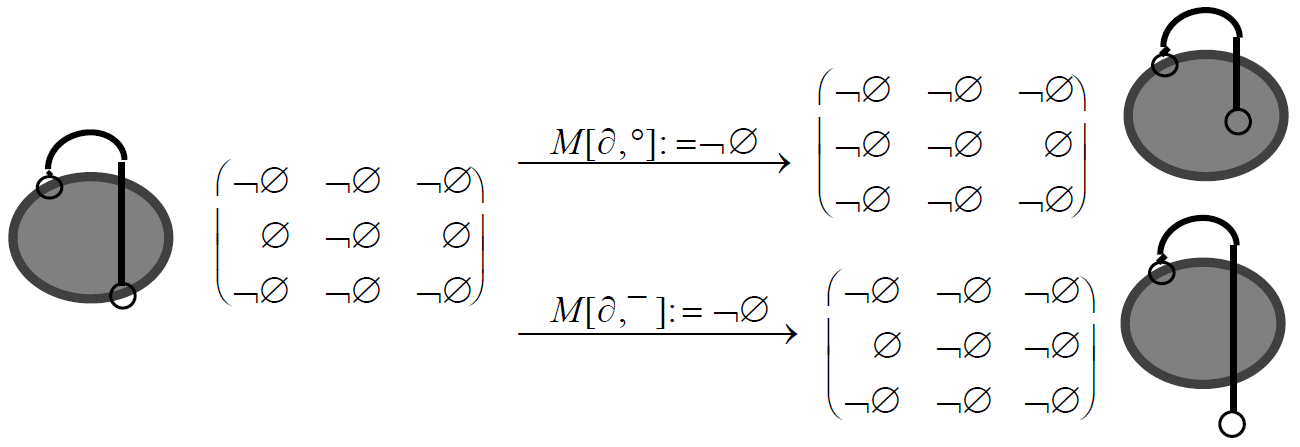
\includegraphics[width=\textwidth]{images/smooth_transitions_example_a.png}
%		\end{block}
%	\end{frame}
%	
%	\begin{frame}{Second Rule}
%		If the line's two boundaries intersect with two different region parts then move either intersection to the adjacent region part.
%		\begin{block}{Formalization}
%			\centering $ \#M[\delta,\_] = 2 \Rightarrow
%			\forall i (M[\delta, i] = \NotEmpty):
%			M_{N}[\delta, i] := \Empty \text{ \textbf{and} }
%			M_{N}[\delta, \text{adjacent}(i)] := \NotEmpty $
%		\end{block}
%		
%		\begin{block}{Example}
%			%Moving either boundary into an adjacent region part.
%			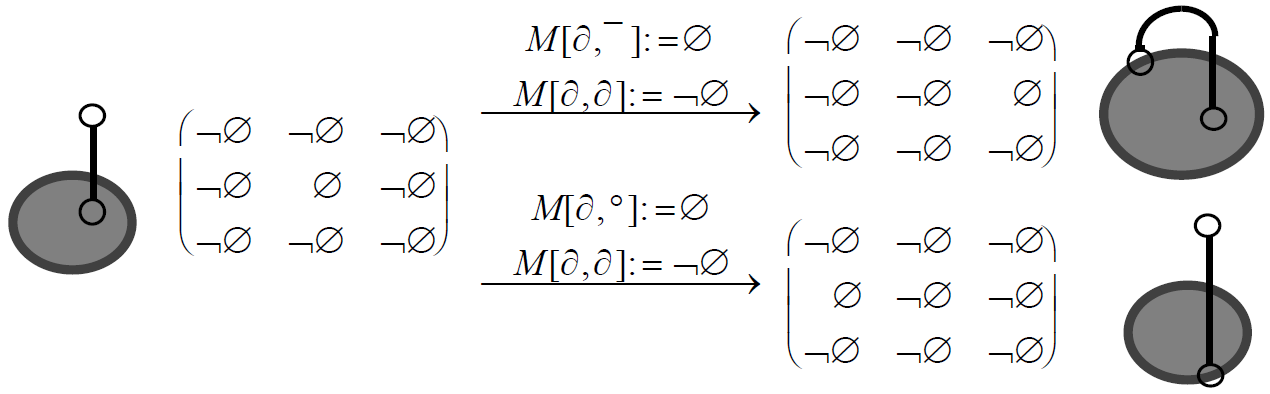
\includegraphics[width=\textwidth]{images/smooth_transitions_example_b.png}
%		\end{block}
%	\end{frame}
%	
%	\begin{frame}{Third Rule}
%		Extend the line's interior-intersection to either of the adjacent region parts.
%		
%		\begin{block}{Formalization}
%			\centering $ \forall i (M[°, i] = \NotEmpty):
%			M_{N}[°, \text{adjacent}(i)] := \NotEmpty $
%		\end{block}
%		
%		\begin{block}{Example}
%			%Moving the line's interior into an adjacent part of the region.
%			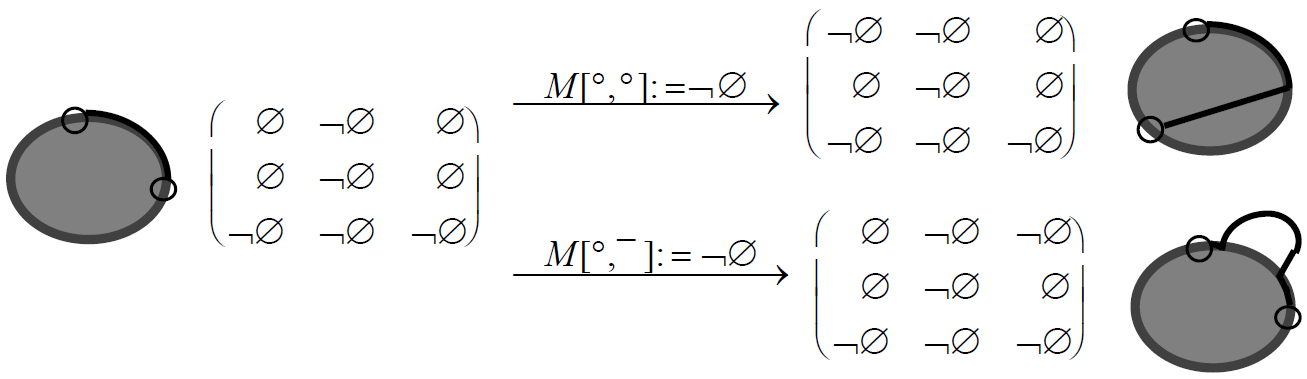
\includegraphics[width=\textwidth]{images/smooth_transitions_example_c.png}
%		\end{block}
%	\end{frame}
%	
%	\begin{frame}{Fourth Rule}
%		Reduce the line's interior intersection on either of the adjacent region parts.
%		
%		\begin{block}{Formalization}
%			\centering
%			$ \#M[°, \_] = 2 \Rightarrow
%			\forall i (M[°, i] = \NotEmpty):
%			M_{N}[°, i] := \Empty $
%			$ \#M[°, \_] = 3 \Rightarrow
%			\forall i (i \neq \delta):
%			M_{N}[°, i] := \Empty $
%		\end{block}
%		
%		\begin{block}{Example}
%			%Moving the line's interior out of a part of the region.
%			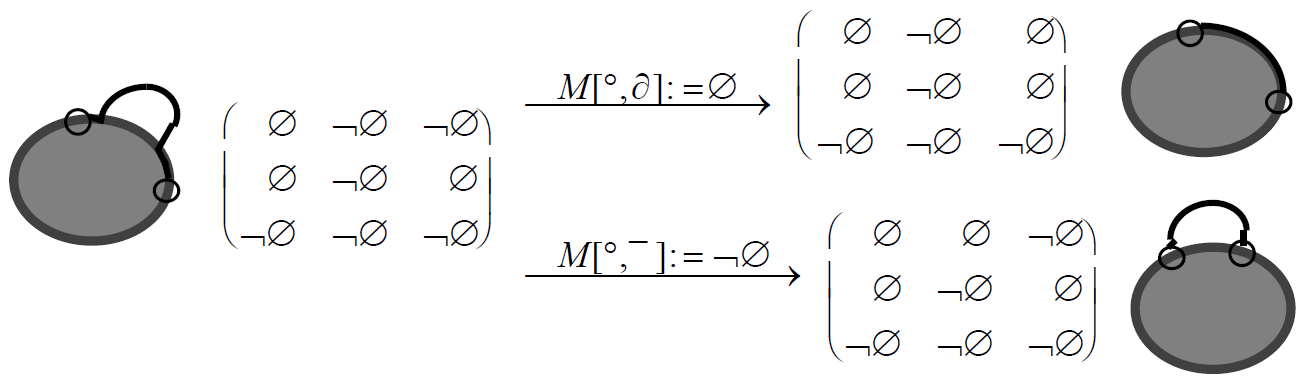
\includegraphics[width=\textwidth]{images/smooth_transitions_example_d.png}
%		\end{block}
%	\end{frame}
%	
%	\begin{frame}{Consistency Constraints}
%		\begin{enumerate}
%			\item If the line's interior intersects with the region's interior \textit{and} exterior, then the line's interior must also intersect with the region's boundary.
%			\begin{center}
%				$ M[°,°] = \NotEmpty \text{and} M[°,^{-}] = \NotEmpty \Rightarrow M[°,\delta] := \NotEmpty $
%			\end{center}
%			
%			\item If the line's boundary intersects with the region's interior (exterior) then the line's interior must intersect with the region's interior (exterior) as well.
%			\begin{center}
%				$ M[\delta, °] = \NotEmpty M[°,°] := \NotEmpty $ \\
%				$ M[\delta, ^{-}] = \NotEmpty M[°,^{-}] := \NotEmpty $
%			\end{center}
%		\end{enumerate}
%		
%	\end{frame}
	
	% NOTES:
	% The separate moves of the line's interior and boundaries are atomic operations that do not account for some of the properties of the objects and their embedding space and, therefore, may generate inconsistent 9-intersections for configurations that cannot be realized. In order to maintain connectivity among the line's boundaries and interior, it is necessary to assure the following \textbf{consistency constraint}: [1]. Likewise, in order to preserve the continuous-space property of $\mathcal{R}^{2}$, the following consistency constraint must be fulfilled: [2].
	
	\begin{frame}{Resulting Neighborhood Graph}
		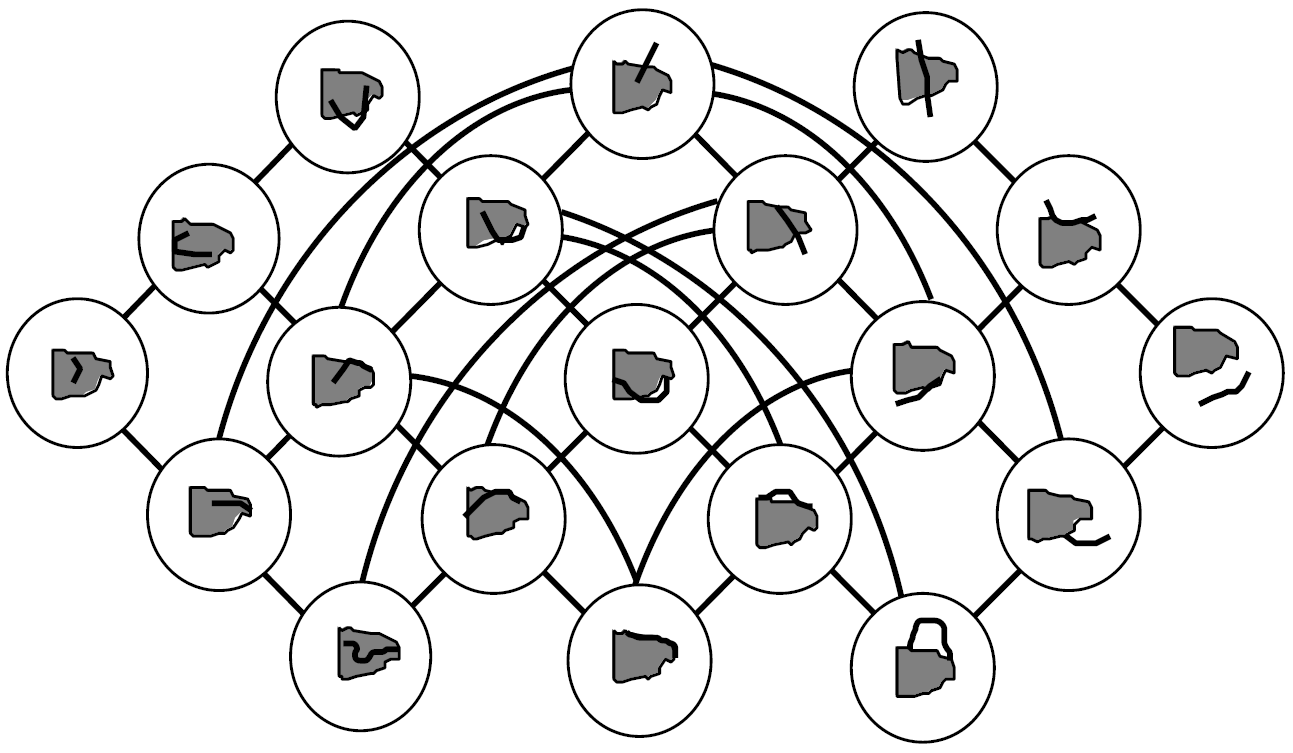
\includegraphics[width=\textwidth]{images/smooth_transitions_neighborhood_graph.png}
	\end{frame}
	
	\begin{comment}
		- images are a bit small
		- the purpose is to give the audience just a feeling of how similar/ different the models are
		- resemble a lot in structure
		- differences are the way in which conceptual neighbors are connected at the to and the additional links that run across the smooth transition graph
	\end{comment}
	
	\begin{frame}{Juxtaposition of Neighborhood Graphs}
		\begin{tabularx}{\textwidth}{XX}
			\begin{center}
				\textbf{Snapshot Model}
			\end{center}
			&
			\begin{center}
			\textbf{Smooth-Transition Model}
			\end{center} \\
			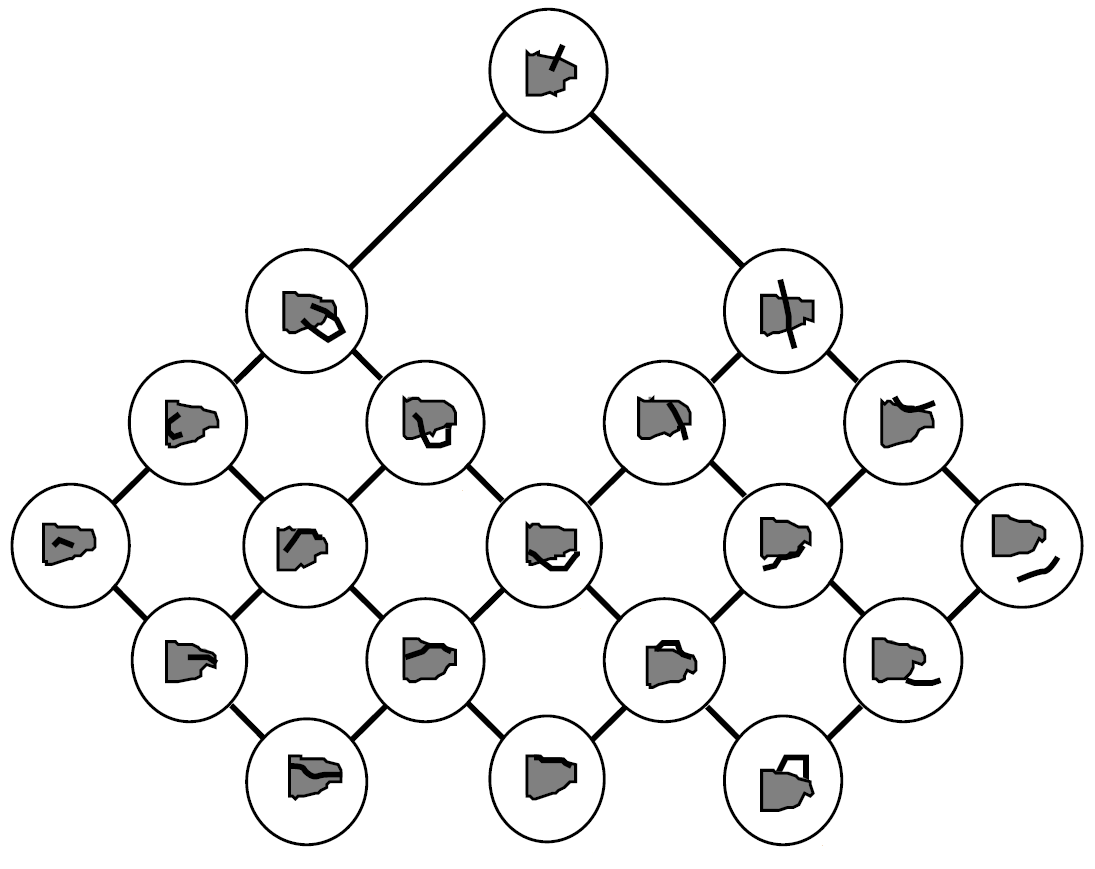
\includegraphics[width=0.48\textwidth]{images/snapshot_model_neighborhood_graph_simple.png}
			&
			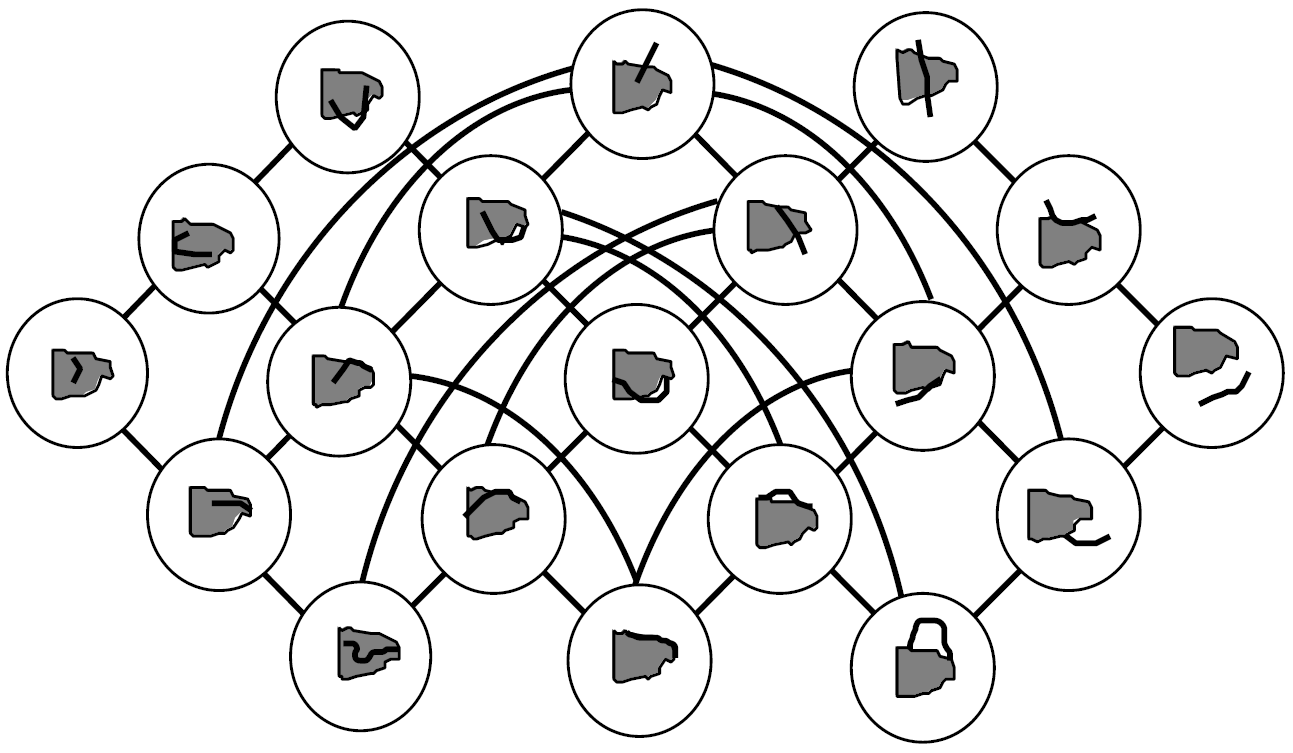
\includegraphics[width=0.48\textwidth]{images/smooth_transitions_neighborhood_graph.png}
		\end{tabularx}
	\end{frame}
	
	\begin{comment}
		\begin{itemize}
		\item 19 line-region relations $\rightarrow$ 171 distinct pairs of relations that can possibly be conceptual neighbors
		\item 26 under snapshot model and the smooth-transition model
		\item 2 under snapshot model
		\item 12 under smooth-transition model
		\item 131 pairs under neither model
		\end{itemize}
	\end{comment}